\section{\texttt{Current work}}
\begin{frame}{\textbf{Saliency Estimation}}
\begin{columns}
	\begin{column}{0.48\textwidth}
		\begin{varblock}[\textwidth]{Objective}
			To identify pixels that are quite distinct and grabs attention.
		\end{varblock}
	\end{column}
	\begin{column}{0.48\textwidth}
	\begin{varblock}[\textwidth]{Techniques}
		\footnotesize
		\begin{multicols}{2}
		\begin{enumerate}[(a)]
    			\item Hierarchical Color Based
    			\item Spectral Distribution Based
		    \item Context Aware Based
    			\item Regional Contrast
		\end{enumerate}
		\end{multicols}			
	\end{varblock}
	\end{column}
\end{columns}
	\begin{figure}
		\centering
		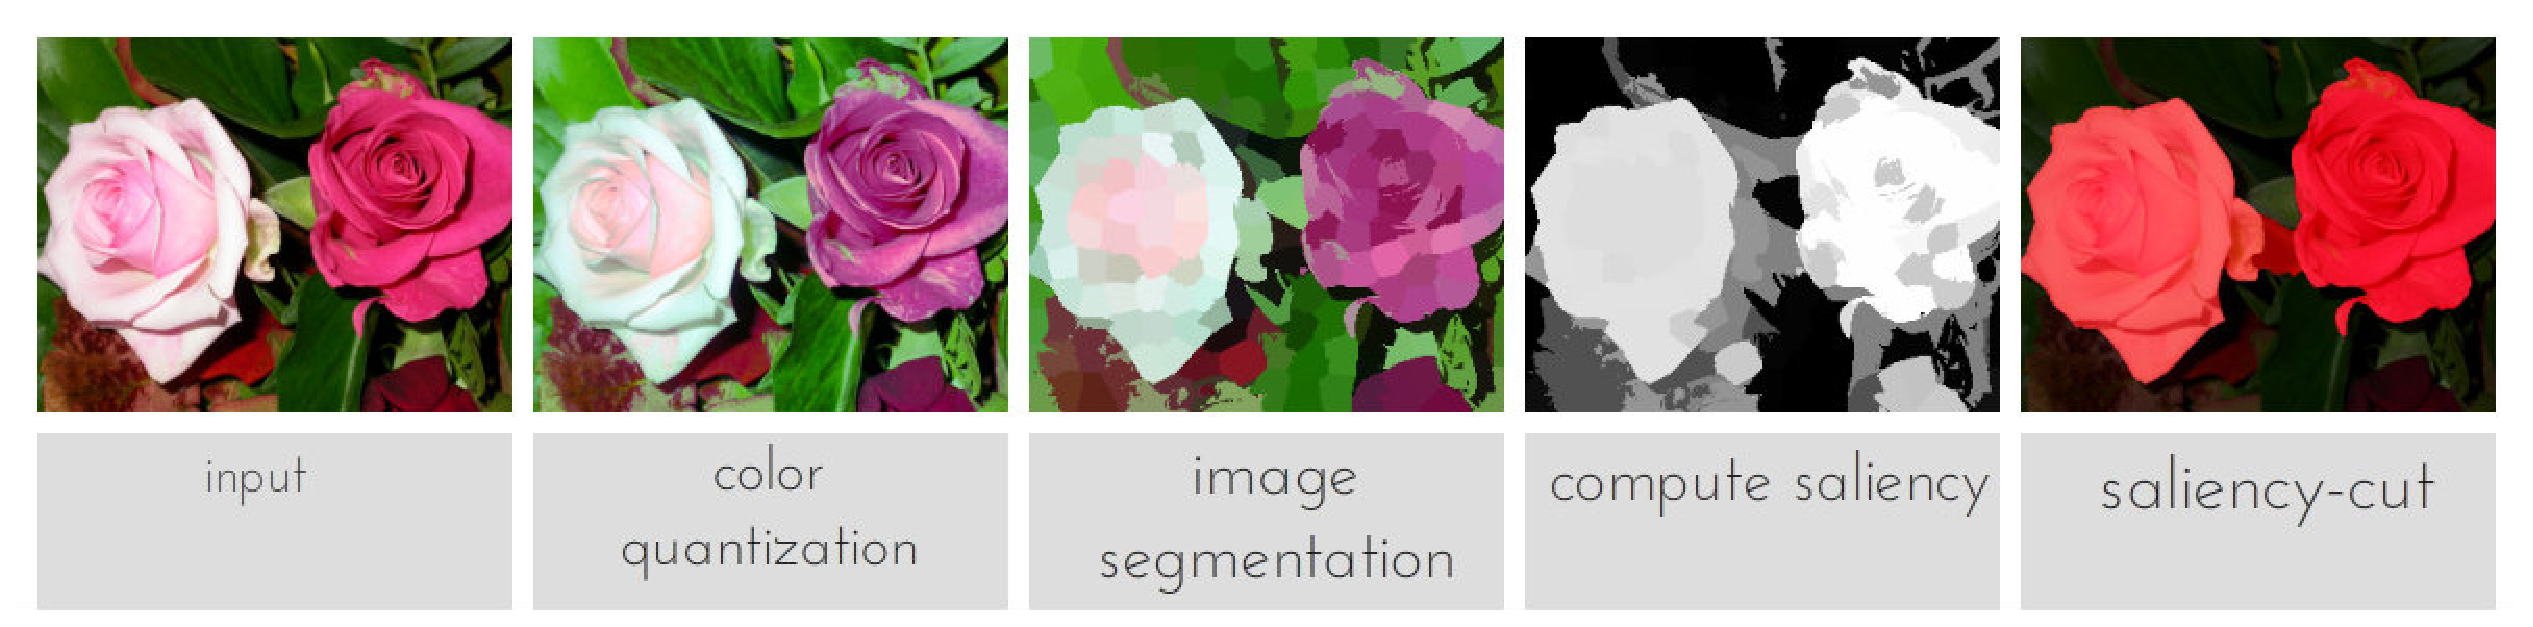
\includegraphics[width=0.7\textwidth]{./img/saliency.eps}
		\caption{A general approach for saliency estimation.}
	\end{figure}
\end{frame}

\begin{frame}{\textbf{Saliency Estimation}}
\begin{figure}
	\fbox{\begin{minipage}{.45\textwidth}		
		\begin{subfigure}[c]{\textwidth}
			\centering
			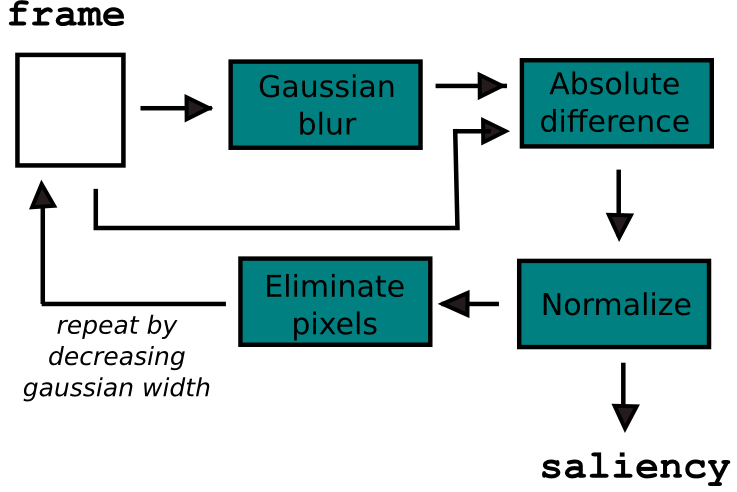
\includegraphics[width=0.65\textwidth]{./img/sal_hcb.png}
			\caption{Hierarchical Color}
		\end{subfigure}
	\end{minipage}}
	\fbox{\begin{minipage}{.45\textwidth}		
		\begin{subfigure}[c]{\textwidth}
			\centering
			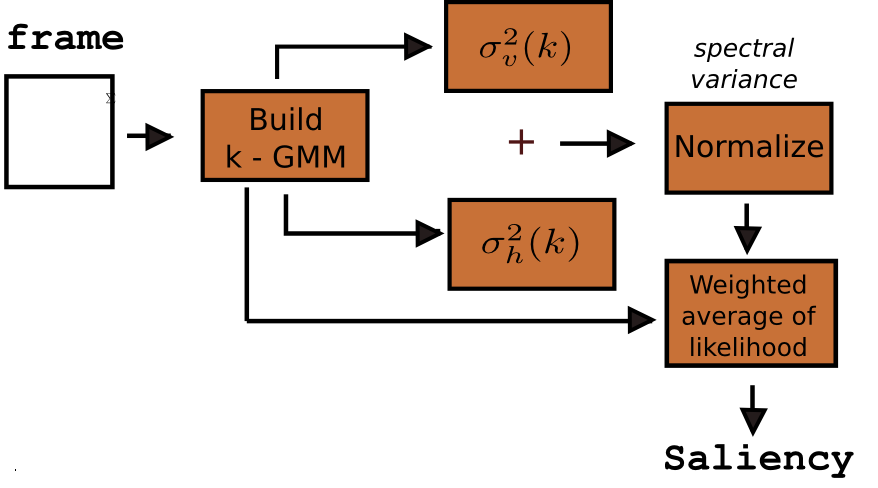
\includegraphics[width=0.78\textwidth]{./img/sal_sdb.png}
			\caption{Spectral Distrbution}
		\end{subfigure}
	\end{minipage}}	
	\fbox{\begin{minipage}{.45\textwidth}		
		\begin{subfigure}[c]{\textwidth}
			\centering
			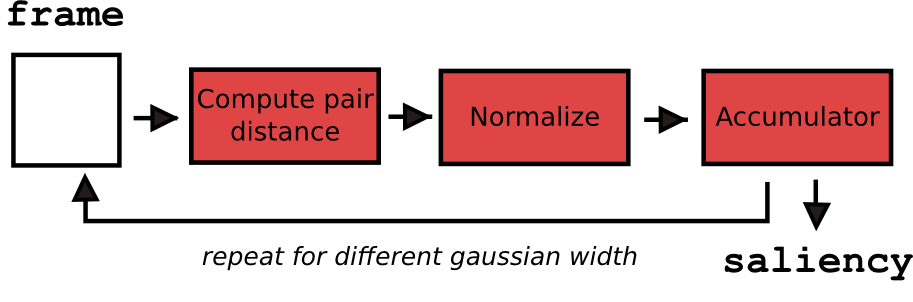
\includegraphics[width=0.90\textwidth]{./img/sal_ca.png}
			\caption{Context Aware}
		\end{subfigure}
	\end{minipage}}
	\fbox{\begin{minipage}{.45\textwidth}
		\begin{subfigure}[c]{\textwidth}
			\centering
			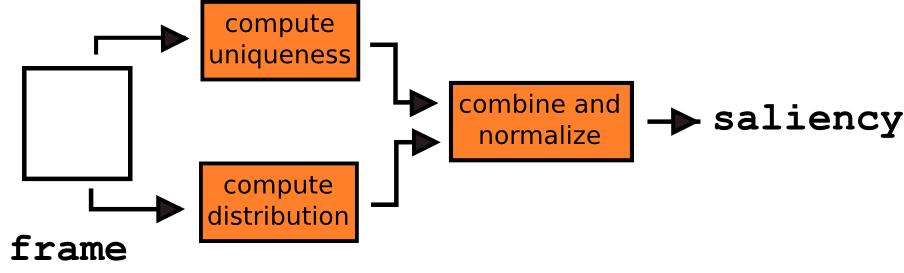
\includegraphics[width=0.94\textwidth]{./img/sal_rc.png}
			\caption{Region Contrast}
		\end{subfigure}
	\end{minipage}}
\end{figure}
\end{frame}

\begin{frame}{\textbf{Saliency Estimation}}
\begin{columns}
	\begin{column}{0.48\textwidth}
		\begin{figure}
		\centering
		\includegraphics[width=\textwidth]{./img/saliencyall.eps}
	\end{figure}
	\end{column}
	\begin{column}{0.48\textwidth}
	\begin{scriptsize}
		\begin{table}[htbp]
		\caption{Results on Weizmann Dataset}
			\begin{subtable}[Single object segmentation]{\textwidth}
			\centering
			\caption{Single object segmentation}
			\begin{tabular}{|l|c|c|c|} \hline
			\textbf{methods} & \textbf{precision} & \textbf{recall} & \textbf{f-measure} \\ \hline
 	    			\emph{HCB} & 0.425 & 0.312 & 0.294 \\
	 			\emph{CAB} & 0.418 & 0.363 & 0.355 \\
 	 			\emph{SDB} & 0.469 & 0.735 & 0.514 \\
	 			\emph{RC}  & {\color{yellow}\textbf{0.772}} & 0.769 & 0.730 \\
	 			\emph{RC~+~D} & 0.703	& {\color{yellow}\textbf{0.862}} & {\color{yellow}\textbf{0.733}}	\\ \hline
   			\end{tabular}
  	 	\end{subtable}
		\hspace{2em}
		\begin{subtable}[Single object segmentation]{\textwidth}
			\centering
			\caption{Multiple object segmentation}			
			\begin{tabular}{|l|c|c|c|} \hline
				\textbf{methods} & \textbf{precision} & \textbf{recall} & \textbf{f-measure} \\ \hline
				\emph{HCB} & 0.396 & 0.434 & 0.339 \\
				\emph{CAB} & 0.573 & 0.475 & 0.473 \\
				\emph{SDB} & 0.360 & 0.674 & 0.392 \\
				\emph{RC}  & {\color{yellow}\textbf{0.763}} & {\color{yellow}\textbf{0.772}} & {\color{yellow}\textbf{0.732}} \\ \hline
   			\end{tabular}
	   	\end{subtable}
 		\end{table} 
	\end{scriptsize}
	\end{column}
\end{columns}
\end{frame}


\begin{frame}{\textbf{Temporal Smoothening}}
\begin{columns}
	\begin{column}{0.48\textwidth}
		\begin{varblock}[\textwidth]{Objective}
			To remove  spurious pixels in the masks obtained because of camera motion, occlusion and illumination variations.
		\end{varblock}
		\begin{varblock}[\textwidth]{Previous Approaches}
			\begin{itemize}
				\item Gaussian Smoothening
				\item Morphological Operations
			\end{itemize}
		\end{varblock}
		\begin{varblock}[\textwidth]{Objective}
				\begin{itemize}
				\item Eigen Based
				\item Semi supervised learning
				\item \textbf{\color{blue}Gausian Mixture Based}
			\end{itemize}	
		\end{varblock}
	\end{column}
	\begin{column}{0.48\textwidth}
	\begin{figure}
		\centering
		\fbox{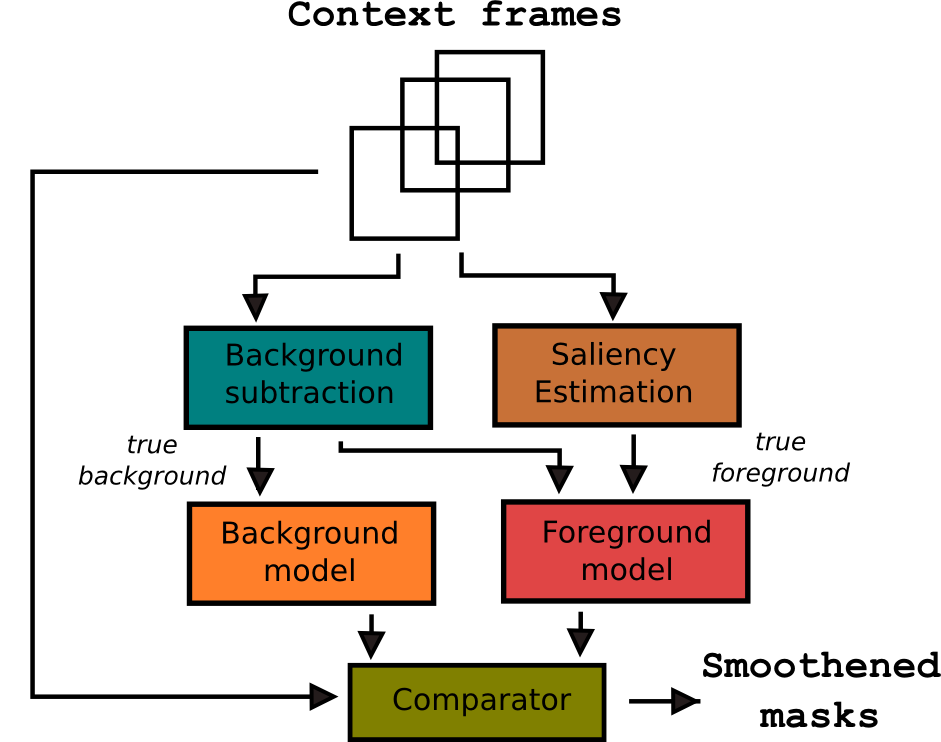
\includegraphics[width=0.95\textwidth]{./img/temporal_smoothening.png}}
		\caption{Approach for Temporal Smoothening.}
	\end{figure}
	\end{column}
\end{columns}
\end{frame}

\begin{frame}{\textbf{Temporal Smoothening}}
\begin{columns}
	\begin{column}{0.48\textwidth}
		\begin{figure}
			\centering
				\includegraphics[width=0.95\textwidth]{./img/example_smoothen.eps}
				\caption{Gaussian Mixture Based Smoothening.}
		\end{figure}
	\end{column}
	\begin{column}{0.48\textwidth}
	  \begin{table}[htbp]
   		\caption{Results on Change Detection Dataset.}
   		\begin{scriptsize} \begin{center}
   		\begin{tabular}{|l|c|c|c|} \hline
       		 \textbf{challenges} & \textbf{precision} & \textbf{recall} & \textbf{f-measure} \\ \hline
				\emph{bad Weather} & 0.16 & 0.78 & 0.26\\
				\emph{baseline} & 0.19 & {\color{yellow}0.83} & 0.28\\
				\emph{camera Jitter} & 0.13 & 0.70 & 0.21 \\
				\emph{dynamic Background} & 0.11 & 0.55 &  0.18\\
				\emph{Object Motion} & 0.11 & 0.62 & 0.18 \\
				\emph{low Frame rate} & 0.14 & 0.44 & 0.20 \\
				\emph{night Videos} & 0.08 & 0.70 & 0.14 \\
				\emph{PTZ }& 0.05 & 0.74 & 0.09\\
				\emph{shadow} & 0.13 & 0.64 & 0.20\\ \hline
 		\end{tabular} \end{center} \end{scriptsize}
 	 \end{table} 
	\end{column}
\end{columns}
\end{frame}

\begin{frame}{\textbf{Tracking}}
\begin{columns}
	\begin{column}{0.48\textwidth}
		\begin{varblock}[\textwidth]{Objective}
			To draw a bounding box around the region of interest and then track them across frames.
		\end{varblock}
		\begin{varblock}[\textwidth]{}
			This ensures robust bounding boxes if there are any uneventful (no mask) or extremely eventful (too many mask) frame based on the history.			
		\end{varblock}
	\end{column}
	\begin{column}{0.48\textwidth}
		\begin{figure}
			\centering
				\fbox{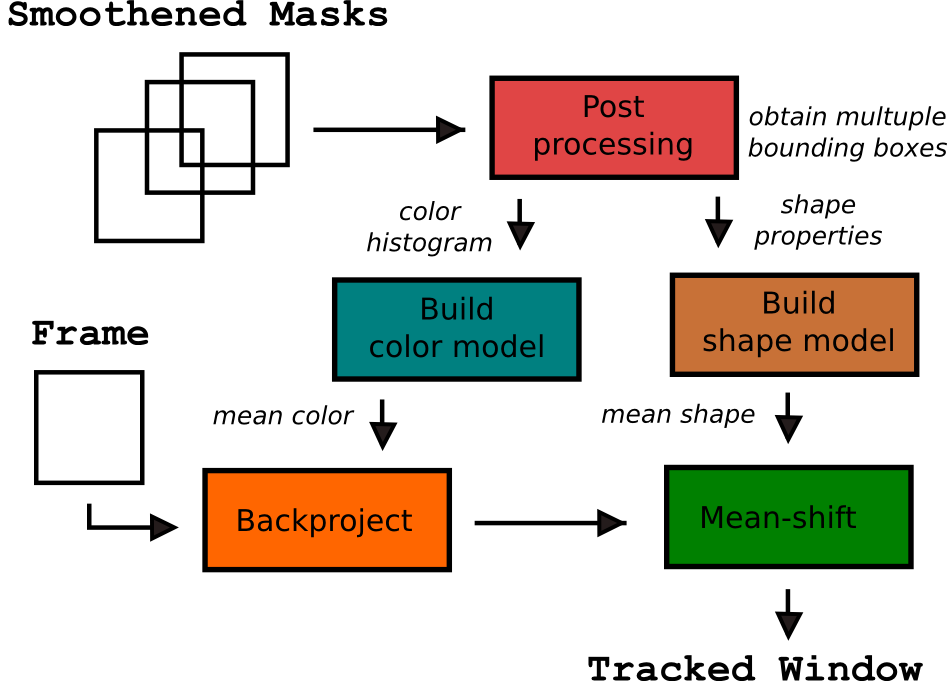
\includegraphics[width=0.95\textwidth]{./img/tracking.png}}
				\caption{Tracking from smoothened mask.}
		\end{figure}
	\end{column}
\end{columns}	
\end{frame}